In order to consider any conception of mathematical fragility, we must first begin to develop the
mathematical context of this project. The following discussion takes place in a probability space, and I
will leave I chose to investigate a special subset of Markov chains known as
birth and death chains. In particular, a Markov chain is defined as follows.
\begin{definition}
    A random process $X(t)$ is called a \emph{Markov chain} if, for any $t_1 < t_2$,
    \[
        P[X(t_2) \leq x \mid X(t) \text{ with } -\infty < t \in \leq t_1] = P[X(t_2) \leq x \mid X(t_1)]   
    \]
\end{definition}
In less formal terms, the probability that the chain assumes a state less than $x$ depends only on the
previous state, and none of the states before it. A birth and death chain is a special subset of Markov
chains in which the probability of stepping away from state $i$ is dependent on the current position of
the chain. A birth and death chain can be thought of as a model of a person walking amidst a fog that
obscures a point of interest. The current state of the chain is thus the current position of the walker.
For the purposes of this project, it made the most sense to consider chains with a state space of $\N$,
as they offered the most simplicity for initial investigation. The following diagram represents a birth
and death chain with state space $\N$.

\noindent
\begin{figure}[H]
    \begin{center}
        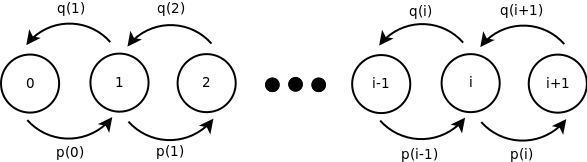
\includegraphics[width=\textwidth]{plots/birthdeathdia.png}
    \end{center}
\end{figure}

Birth and death chains are suitable context for this project due to the fact that they can model a wide
range of scenarios in a variety of different fields. Thus, mathematical fragility developed for
arbitrary birth and death chains will allow the conception of fragility to be applied in real world
scenarios. Further, there are a number of quantities associated with birth and death chains that could
provide information about the perceived fragility of these chains.
